\documentclass[a4paper,11pt,oneside]{article}
%Packages
\usepackage{amsmath}
\usepackage{graphicx}
\usepackage{fullpage}
\usepackage{graphicx}
\usepackage{tikz}
\definecolor{lichtgrijs}{gray}{0.95}
\setlength{\parskip}{\baselineskip}%vertical line spacing by new paragraph
\setlength{\parindent}{0cm}
\usepackage[english]{babel}
\usepackage{pgfplots}
\usepackage{gnuplot-lua-tikz}
\usepackage{epstopdf}
\epstopdfsetup{outdir=./}
\usepackage{algorithmic}
\usepackage{algorithm}
\usepackage{enumerate}
\usepackage{geometry}
\usepackage{caption}
\usepackage{chngpage}
\usepackage{tikz}
\usetikzlibrary{chains}
\usepackage{eurosym}
\def\arraystretch{1.5}
\usepackage{wrapfig}
\usepackage{enumitem}
\setlist[itemize]{noitemsep, topsep=2pt}
\setlist[enumerate]{noitemsep, topsep=2pt}
\usepackage{wrapfig}
\usepackage{subcaption}
\usepackage{import}

\usepackage[numbers]{natbib}

\usepackage{url}
%\usepackage[round]{natbib} % Voor auteur-jaar citaties
\bibliographystyle{bibliodutch}
\usepackage[nottoc]{tocbibind} % Bibliografie in ToC; zie tocbibind.dvi

\usepackage[toc,page]{appendix}

%Listings
\usepackage{listings}
\lstset{
	basicstyle=\scriptsize,
	backgroundcolor=\color{lichtgrijs},
	numbers=left,
	numberstyle=\tiny,
	numbersep=9pt,
	showspaces=false,
	showstringspaces=false,
	showtabs=false,
	frame=leftline,
	tabsize=2,
	captionpos=b,
	title=\lstname,
	breaklines=true,
	breakatwhitespace=true,
	stepnumber=4
}
\lstdefinestyle{customc}{
  belowcaptionskip=1\baselineskip,
  breaklines=true,
  language=R,
  showstringspaces=false,
  basicstyle=\footnotesize\ttfamily,
  keywordstyle=\bfseries\color{green!40!black},
  commentstyle=\itshape\color{purple!40!black},
  stringstyle=\color{orange},
}

\begin{document}

%  Titelblad

% Opmerking: gaat uit van een \baselinestretch waarde van 1.5 (die moet
% ingesteld worden voor het begin van de document environment)

\begin{titlepage}
\pagenumbering{gobble}% Remove page numbers (and reset to 1)
\clearpage
\newgeometry{top=2cm, bottom=2cm, right=1.5cm, left=1.5cm}

%logo
\begin{figure}[!ht]
  \begin{adjustwidth}{-1.5cm}{}
    \centering
    
\includegraphics[width=\paperwidth]{logo.jpg}
  \end{adjustwidth}
\end{figure}

\begin{center}

\fontsize{12pt}{14pt}
\selectfont
 
\vspace{6cm} 
\Huge \textsc{Design of Multimedia Applications:}\\ 
\vspace{1cm}
\huge
\textsc{Video Shot Detection, Annotation,\\ and Retrieval}\\
\vspace{10.5cm}
\Large
Group 40:\\
Eveline Hoogstoel, Titouan Vervack and Dries Wijns\\
$1^{st}$ Master in Computer Science Engineering


\end{center}
\end{titlepage}

\thispagestyle{empty}

\pagebreak

\newgeometry{left=2.5cm,right=2.5cm,bottom=2.5cm, top=2.5cm}
\pagenumbering{arabic}% Arabic page numbers (and reset to 1)

\section{Explanation of the used algorithms.}
\subsection*{Exercise 2.B}
For the implementation of exercise 2.B we have first calculated the distances of the pixels left, right, above and below the pixel. Once we know these distances it is easy to get the 2 lowest numbers. The distances were stored in an array, so once we have determined on which index the two lowest values are stored we know exactly which pixel it is. We can indicate which pixels are taken with extra boolean values (\verb!t_taken!, \verb!b_taken!, \verb!r_taken! and \verb!l_taken!), by initialisation of these values we take into account whether the macroblock exists or not. In the formula for the calculation of the luma- or chrominancevalue we multiply each term by it's corresponding boolean, so we know if we have to take the value of that pixel into account or not.

\subsection*{Exercise 2.C}
First of all it should be said that we were unable to finish this exercise. We were able to do edge detection but adding actual extrapolation was outside of our capabilities. Nevertheless we'll try to discuss what we were unable to make in pseudocode and try to predict it's results. We also did measurements for this exercise but these are of course not as they should be.\\
For this assignment we first do edge detection and with the information gained from this we extrapolate the missing macroblock. The technique that we used for edge detection is the Sobel operator. We chose this technique over various others, i.e. Canny, because it gives a good result and is more accurate for corners than Canny is. It is  also one of the easier ones to implement. It's disadvantage is that Canny performs better. Sobel is also used in Canny which gave us the ability to use Canny later on.\par
We started off by looping over all macroblocks in the frame and for those missing we collected the four macroblocks around it. From these macroblocks we take the three rows or columns closest to the missing macroblock, this in order to simplify the calculations and reasoning. On every pixel's lumavalue (because when we purely consider the lumavalues of an image we actually have it's grayscale)   of these  simplified macroblocks we ran the Sobel operator. The dotproducts needed in Sobel are done by creating a 3x3 block with the current pixel in the middle. Using Sobel we can also calculate the gradient's direction. In order to simplify this we grouped these directions according to the 8 wind directions. We also save the pixels with the same direction in a list so that we can decide where the edge starts later on.\par
This is about how far we were able to get so we will now discuss what our further plans with this were. From here on we would've checked if there were three pixels (in the three different rows/columns) with the same direction that were aligned in such a way that they'd form an edge. If less than three were found we decide that no edge was found. We do this for all blocks and then we check the found edges with all the others to see if two of them could be connected. Once that is done all we have to do is fill in the planes between the extrapolated edges.\\
\begin{lstlisting}[frame=single]
void conceal_spatial_3(frame)
{
for (int i = 0; i < frame->getNumMB(); i++) {
    if(frame->getMacroBlock(i)->isMissing()){
	    // Get the blocks left, right, above and below the missing block
	    blocks = getNeighbouringBlocks();
	    // Only get the 3 rows or columns that border to the macroblock
        sides = getSides(blocks);
        edges = sobel(sides);
        extrapolate(edges, sides);
	}
}

short horizontal_sobel[3][3] = {
		{ -1, 0, 1 },
		{ -2, 0, 2 },
		{ -1, 0, 1 }
};

short vertical_sobel[3][3] = {
		{ 1, 2, 1 },
		{ 0, 0, 0 },
		{ -1, -2, -1 }
};

edge* sobel(sides){
	// The 8 wind directions in degrees: 0, 45, 90, 135, ...
	int direction[8] = { 0 };
	// The pixels where we detected the angles
	list<list<pair<int, int>>>  indices = new list(8, list<pair<int, int>>(3 * 16));
	for (pixel in side){
		for (3x3Block)
			if (partOf3x3Block.outOfBounds()){ continue; }
			
			gx = 3x3Block->luma.dotProduct(horizontal_sobel);
			gy = 3x3Block->luma.dotProduct(vertical_sobel);
		}
		double g = sqrt((gx*gx + gy*gy) / 8);
		double angle = atan2(gy, gx) * 180.0 / PI;

		direction[floor(angle / 45)] += g;
		// Remember which pixel has what angle
		indices[a].add(pair<int, int>(i, j));
    }
    
	// Return the edge, contains it's angle and the pixels that have this angle
	edge *e = new edge;
	e->direction = direction;
	e->indices = indices;

	return e;
}

void extrapolate(edges, sides){
    for (side in sides) {
        for (otherside in sides) {
            // Loop over de edges that are in side
            // we can determine this from the "indices" we calculated above
            for (edge in side) {
                for (otherEdge in side) {
                    // Check if the direction of the edge is the opposite of the other edge
                    // this means they can be connected
                    if (edge.oppositeWindDirectionFrom(otherEdge)) {
                        extrapolateMacroblock();                    
                    }                
                }            
            }        
        }    
    }
}
\end{lstlisting}

Since we were unable to complete this assignment our quality and time measurements are incorrect.
\subsection*{Exercise 3.B}
\vspace{-0.5cm}
To allow for submacroblock concealing, we first build a list of the macroblock movement vectors of neighboring macroblocks.
We then build a list of submacroblock movement vectors that span a whole macroblock, f.ex. if submacroblock size is 8 by 8 pixels, 
then the submacroblock movement vectors are (0,0), (1,0), (0,1) and (1,1).

For a missing macroblock we do the following algorithm:
\begin{lstlisting}[frame=single]
let mmvs be the list of macroblock movement vectors
let smvs be the list of submacroblock movement vectors

initialize best_mmv to none
initialize best_smv to none
initialize smallest_error to +inf

for each submacroblock in the missing macroblock:
	for each mmv in mmvs:
		for each smv in smvs:
			total_movement_vector = 16*mmv + submacroblock_width*smv
			compute error 
			if error < smallest_error:
				smallest_error = error
				best_smv = smv
				best_mmv = mmv

replace submacroblock by submacroblock pointed to by best_smv and best_mmv
\end{lstlisting}
\vspace{-1.2cm}
\subsection*{Exercise 3.C}
\vspace{-0.5cm}
To allow for missing neighboring macroblocks we had to do one small improvement on exercise 3.B:
instead of conceiling missing macroblocks in the order they occur in the frame,
we select the macroblock that has the most available neighboring macroblocks and conceil him first.

By doing this, clusters of missing macroblocks will be conceiled from the edges to the center.

\subsection*{Exercise 3.D}
\vspace{-0.5cm}
Adaptive submacroblock conceiling has been done with a recursive algorithm.\\
For each missing macroblock (in the same order as 3.C) we do:
\begin{lstlisting}[frame=single]
function conceil_submacroblock(submacroblock):
	if submacroblock_width > 2 pixels:
		split the submacroblock into 4 quarters: q0, q1, q2, q3
		recursivly call conceil_submacroblock on each quarter, resulting in 4 error measures e0, e1, e2, e3
		
		calculate the error measure e when conceiling the full submacroblock
		
		if e < min(e0, e1, e2, e3):
			conceil the full submacroblock
			return e
		else:
			return min(e0, e1, e3, e3)
	else:
		calculate the error measure e when conceiling the full submacroblock
		conceil the full submacroblock
		return e
\end{lstlisting}
\vspace{-1cm}
The error measures e, e0, e1, e2 and e3 are the mean error over the boundary pixels. \\
The first call to this function is done with a submacroblock size 16 by 16 pixel, the full macroblock size.\\

\section{Measurement results}
\vspace{-0.5cm}
\subsection*{Test platform}
\vspace{-0.5cm}
All of our test were run on the following hardware and software:
\begin{itemize}
	\item \textbf{CPU:} Intel I7 2600k quad core @3.9Ghz
	\item \textbf{RAM:} Corsair Vengeance 8GB (2x4GB) CL9 @1600Mhz
	\item \textbf{SSD:} Kingston HyperX 3K 240GB, 555MB/s sequential read, 85.000 IOPS (4K random reads) (used for reading) 
	\item \textbf{HDD:} Western Digital Blue 1TB 7200RPM 64MB cache (used for writing)
	\item \textbf{OS:} Windows 8.1 Pro 64-bit\\
\end{itemize}
\vspace{-1cm}
\subsection{Quality measurements}
\vspace{-0.5cm}
First of all we have used the PSNR-metric to measure the quality of our video sequences. The results of this quality measurement can be found in figure \ref{fig:PSNR}.\\
\vspace{-0.7cm}
\begin{figure}[H]
\subimport{VQMT/}{psnr.tex}
\caption{PSNR values for the 3 video sequences, each decoded with their 2 different errorfiles.}
\label{fig:PSNR}
\end{figure}
\vspace{-0.5cm}
The first thing we notice in this graph is the big difference between the PSNR-values of the video sequences decoded with the simple errorpattern and the video sequences decoded with the complex errorpattern. This is rather obvious because the complex errorpattern introduces more errors.\\
The second thing we notice on this graph is that spacial error concealment implemented in 2B has a much better quality in comparison with the other methods. This is because our natural fragment is quite static, it doesn't move much. The synthetic fragment and the one unique to our group have a lot of movement which makes the error prediction harder resulting in a lower quality and thus a lower PSNR.

We also see that there is basicly no difference in the PSNR for the 3* series. From this we can conclude that the complexity 3D introduces is not worth it.

\paragraph{Beowulf}
\begin{center}
\vspace{-1cm}
\begin{tabular}{c|c|c|c}
2B&2C&3C&3D\\
\hline
32.643326&22.534493&22.534493&22.534493
\end{tabular}
\end{center}
\vspace{-0.5cm}
In the above table we see the PSNR values of the entire Beowulf sequence for the complex errorpattern. We can see 2B has the highest value, so the quality would be better. But we have to mention the value for 2C is not representative. We assume this has to be at least the same psnr value or even better.

\par In figure \ref{fig:SSIM} you can find the SSIM values for all video sequences.
\begin{figure}[H]
\subimport{VQMT/}{ssim.tex}
\caption{SSIM values for the 3 video sequences, each decoded with their 2 different errorfiles.}
\label{fig:SSIM}
\end{figure}
\paragraph{Correlation PSNR and SSIM}
\vspace{-0.5cm}
The SSIM is clearly different from the PSNR for the complex errorpatterns, yet hardly for the simple ones. SSIM gives a correct prediction of the quality for the fragments in 2B, 2C and 3A but not really for 3C and 3D. The distance between the former and the latter has gained in size, but as we visually confirmed, this is the opposite of our actual result.

\subsection{Time measurements}
\vspace{-0.5cm}
In figure \ref{fig:time} you can find the results for the time measurements.
\begin{figure}[H]
\subimport{VQMT/}{times.tex}
\caption{Execution time for decoding the 3 video sequences, each decoded with their 2 different errorfiles.}
\label{fig:time}
\end{figure}

\paragraph{Complexity reduce in 2A and 2B}
We have measured the decoding time with concealing method 0 and 1, once without the optimalisation and once with. In tabel you can see the results of this measurement.
\vspace{-0.5cm}
\begin{center}
\begin{tabular}{ll||c|c||c|c}
&&\multicolumn{2}{c}{2A}& \multicolumn{2}{c}{2B}\\\cline{3-6}
&& 4 pixels & 2 pixels & 4 pixels & 2 pixels\\
\hline
Beowulf & simple & 145.42 & 144.59 & 144.15 & 145.60\\
&complex &/ &/ & 145.60 & 145.66\\
\hline
Elephant & simple & 224.51 & 223.45 & 224.82& 228.30\\
&complex & / &/ & 225.22 & 229.38\\
\hline
Rising times & simple & 85.48 & 86.10 & 86.05& 86.57\\
&complex & / &/ & 85.94 & 86.79\\
\end{tabular}
\captionof{table}{Time measurements (ms)}
\end{center}
\vspace{-0.5cm}
We can see in this table in most cases the computation time goes up for a little bit. Of an algorithmic point of view this is logic because we have to do more checks.


\vspace{-0.5cm}
\subsection{Visual inspection}
\vspace{-0.5cm}
\subsubsection*{Exercise 3.B}
\begin{figure}[H]
        \begin{subfigure}[h]{0.5\textwidth}
                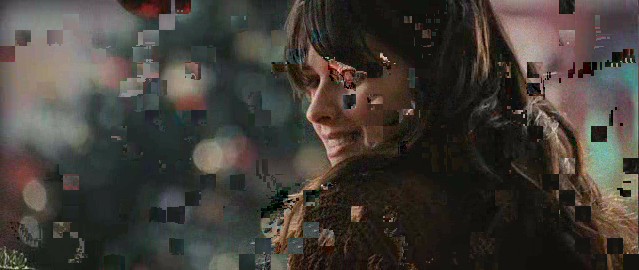
\includegraphics[width=\textwidth]{img/3B_2.png}
                \caption{2 x 2 pixels}\label{subfig:2}
        \end{subfigure}%
        ~
        \begin{subfigure}[h]{0.5\textwidth}
                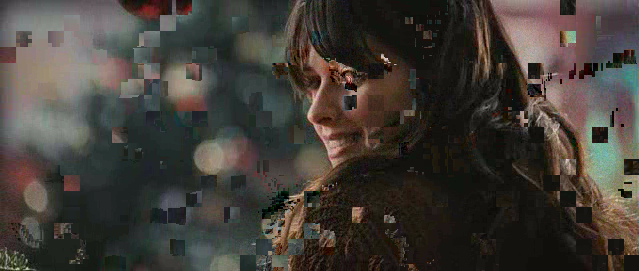
\includegraphics[width=\textwidth]{img/3B_4.png}
                \caption{4 x 4 pixels}\label{subfig:4}
        \end{subfigure}
        ~
        \begin{subfigure}[h]{0.5\textwidth}
                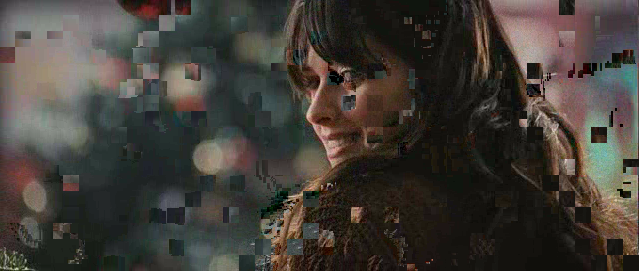
\includegraphics[width=\textwidth]{img/3B_8.png}
                \caption{8 x 8 pixels}\label{subfig:8}
        \end{subfigure}
        ~
        \begin{subfigure}[h]{0.5\textwidth}
                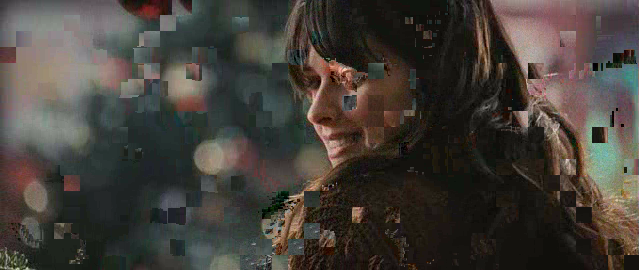
\includegraphics[width=\textwidth]{img/3B_16.png}
                \caption{16 x 16 pixels}\label{subfig:16}
        \end{subfigure}
        \caption{Exercise 3B (simple errorpattern)}\label{fig:ex3B}
\end{figure}
\vspace{-0.5cm}
For the implementation of exercise 3B we have a visual inspection to see what the effect is of using sub-macroblock or not. In figure \ref{fig:ex3B} you can screenshots of frame 10 in  the video sequence \verb!theseekerdarkrising!.\\
If we take a look at the background in the upper left and upper right corner, we can conclude using macroblocks (figure \ref{subfig:16}) is better in comparison of using sub-macroblocks. But on the other hand if we take a look at the eye of the girl, we can conclude figure \ref{subfig:8} has the best reconstruction of the image.\\
So sometimes it can be useful to take a sub-macroblock instead of a macroblock for this conceal method. With this observation we can assume an adaptive implementation will have a better result. But as we can see in figure \ref{fig:3D_simple} this is not much better.
\begin{figure}[H]
\centering
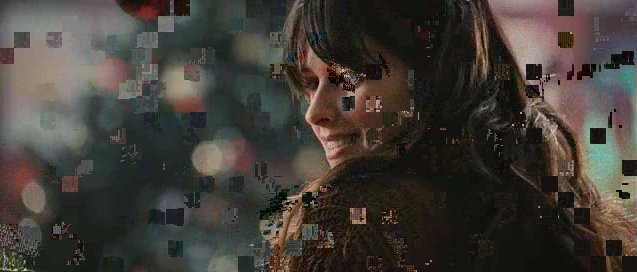
\includegraphics[width=0.5\textwidth]{img/3D_simple.png}
\caption{exercise 3D (simple errorpattern)}\label{fig:3D_simple}
\end{figure}
\vspace{-1cm}
\subsubsection*{Comparision of ex 3A, 3C and 3D}
\begin{figure}[h]
        \begin{subfigure}[h]{0.5\textwidth}
                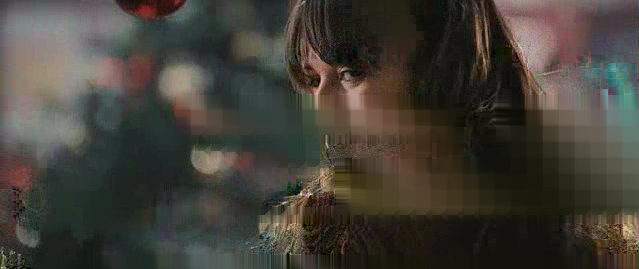
\includegraphics[width=\textwidth]{img/2B_complex.png}
                \caption{exercise 2B}\label{subfig:2B}
        \end{subfigure}%
        ~
        \begin{subfigure}[h]{0.5\textwidth}
                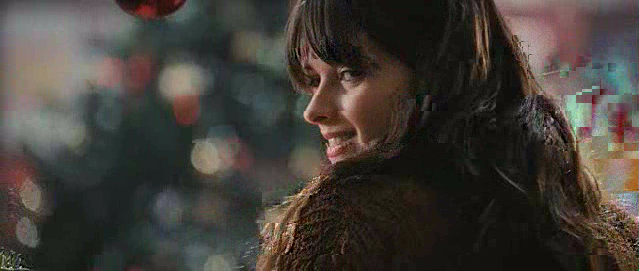
\includegraphics[width=\textwidth]{img/3A_complex.png}
                \caption{exercise 3A}\label{subfig:3A}
        \end{subfigure}
        ~
        \begin{subfigure}[h]{0.5\textwidth}
                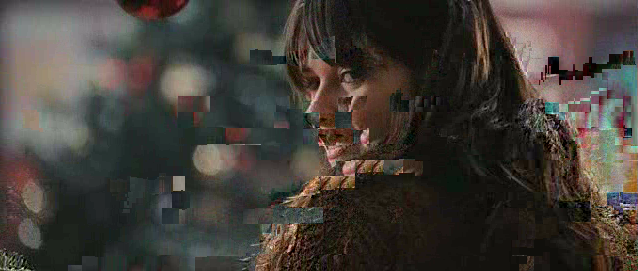
\includegraphics[width=\textwidth]{img/3C_complex.png}
                \caption{exercise 3C}\label{subfig:3C}
        \end{subfigure}
        ~
        \begin{subfigure}[h]{0.5\textwidth}
                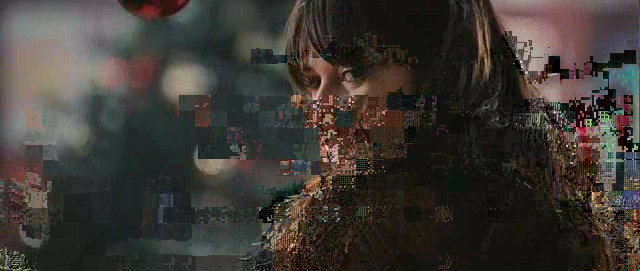
\includegraphics[width=\textwidth]{img/3D_complex.png}
                \caption{exercise 3D}\label{subfig:3D}
        \end{subfigure}
        \caption{Comparision of exercises 3.x (with complex errorpattern)}\label{fig:ex3x}
\end{figure}
\vspace{-0.5cm}
In figure \ref{fig:ex3x} we can see some screenshots of video sequence  \verb!theseekerdarkrising!. Again this pictures are taken on frame 10. On figure \ref{subfig:2B} you can see this frame has a lot of missing macroblocks.\\
If we observe this pictures we can say figure \ref{subfig:3A} is the best. But we have to mention this is because the movement the girl makes is slow. Further in the video we can see more errors when there are bigger motions.\\
When we look at the result of 3D this is not so good. We assumed this would be a little bit better but it is worse.

\section*{Conclusion}
\vspace{-0.5cm}
As said before, we notice that the PSNR values for 2B are a little better when using the complex errorpattern. When we use the simple pattern no real change is noticeable. We would say that 2B is the clear winner but we don't actually have real results for 2C. We'd expect 2C to perform better than 2B, at the cost of a higher complexity and decoding time. Those are also the reasons why we might not choose this technique.\\
Visually we can see the temporal prediction does better than the spatial, which is the opposite of what we just concluded. From this we can learn that just the PSNR value is not enough to decide what fragment has the best quality. People are subjective and different kinds of distortions in images might or might not allow us to still see the image, even if it's PSNR would be low.
\section*{Client-side buffering}
\vspace{-0.5cm}
The main advantage of client-side buffering is that you can perform (better) temporal error concealment. We have seen in our quality measurement that this will help us to better predict the missing macroblocks, so you will have a better user experience. If you are not doing client-side buffering you can only perform spatial error concealment. The disadvantage is that this buffering requires space.

\end{document}


